\chapter{La ecuación de Khokhlov–Zabolotskaya–Kuznetsov}\label{chapter.kzk}
\begin{flushright}
Shock waves, bones to dust\\
You're messin' with a mine field\\
so expect the worst\\
\emph{- Judas Priest (Hard as Iron)-}
\end{flushright}

La ecuación Khokhlov–Zabolotskaya–Kuznetsov (KZK) fue derivada originalmente como una herramienta para la descripción de rayos acústicos no lineales dentro de un medio. Describe la propagación no lineal de un pulso de amplitud finita de un haz de sonido en un medio termo-viscoso. La ecuación, describe con exactitud el proceso entero de auto-demodulación de una señal ultrasónica, a lo largo del campo cercano y hacia el campo lejano. ...
\section{Derivación de la ecuación KZK} 
 Las fuentes de ultrasonido generan fenómenos muy marcados de difracción, que se combinan con los efectos de amplitud finita para producir formas de onda que varían de un punto a otro dentro del haz de sonido. El énfasis en esta sección es la derivación de la ecuación KZK. Se puede probar, en el artículo de Rozanova-Pierrat \cite{mathkzk}, que el problema de la ecuación KZK ...
\begin{figure}[hbpt]
\centering
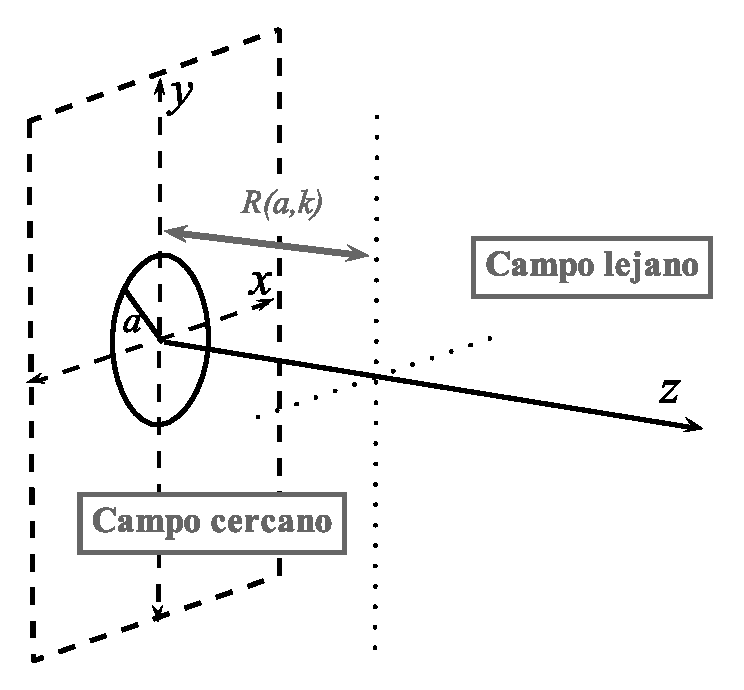
\includegraphics[scale=0.5]{ejepropagacion}
\caption{Esquema del eje de propagación y el radio de la fuente.}
\label{fig:propagacion}
\end{figure}
Normalmente, se caracteriza al campo sonoro de una forma muy similar a los campos electromagnéticos, ya que se clasifican con respecto a la cercanía a la fuente en campo cercano y lejano. Éste, empezando aproximadamente en la distancia de Rayleigh $R(a,k) = (ka^2)\slash2$, medida desde la...
\begin{align*}
& \tildeps\frac{1}{c_0^2}\frac{\partial^2p}{\partial \tau^2} +\tildeps\frac{\delta}{c_0^4}\frac{\partial^3p}{\partial \tau^3}  = -\tildeps^2\frac{\beta}{\rho_0c_0}\frac{\partial^2p^2}{\partial \tau^2}\text{,}
\end{align*}
entonces:
\begin{align*}
&\tildeps\left[ \tildeps\left(\frac{\partial^2}{\partial x_1^2} +\frac{\partial^2}{\partial y_1^2}\right) + \tildeps^2 \frac{\partial^2}{\partial z_1^2} - \tildeps\frac{2}{c_0} \frac{\partial^2}{\partial z_1\partial \tau} +\frac{1}{c_0^2}\frac{\partial^2}{\partial \tau^2}\right]p - = \\
&\quad=-\tildeps^2\frac{\beta}{\rho_0c_0}\frac{\partial^2p^2}{\partial \tau^2}-\tildeps\frac{1}{c_0^2}\frac{\partial^2p}{\partial \tau^2} - \tildeps\frac{\delta}{c_0^4}\frac{\partial^3p}{\partial \tau^3}\text{,}
\end{align*}
de donde se sigue que:
\begin{align*}
&\left[\tildeps^2\left( \frac{\partial^2}{\partial x_1^2}+\frac{\partial^2}{\partial y_1^2}\right) + \tildeps^3\frac{\partial^2}{\partial z_1^2} - \tildeps^2 \frac{2}{c_0}\frac{\partial^2}{\partial z_1\partial \tau} +\frac{1}{c_0^2}\frac{\partial^2}{\partial \tau^2}\right]p - = \\
&\quad = -\tildeps^2\frac{\beta}{\rho_0 c_0}\frac{\partial^2p^2}{\partial \tau^2} - \tildeps\frac{1}{c_0^2}\frac{\partial^2p}{\partial \tau^2} -\tildeps\frac{\delta}{c_0^4}\frac{\partial^3p}{\partial \tau^3}\text{.}
\end{align*}
%
Únicamente es necesario eliminar de los cálculos el término de orden $O(\tildeps^3)$ para quedar con la ecuación siguiente:
%
\begin{align}
\tildeps\left( \frac{\partial^2}{\partial x_1^2} +\frac{\partial^2}{\partial y_1^2}\right)p +\frac{1}{c_0^2}\frac{\partial^2p}{\partial \tau^2} - \frac{1}{c_0^2}\frac{\partial^2p}{\partial \tau^2} - \tildeps \frac{2}{c_0}\frac{\partial^2p}{\partial z_1\partial \tau}+ \frac{\delta}{c_0^4}\frac{\partial^3p}{\partial \tau^3} = -\frac{\beta}{\rho_0 c_0}\frac{\partial^2p^2}{\partial \tau^2}\text{,}\nonumber \\
-\frac{c_0}{2}\times\left[\tildeps\left( \frac{\partial^2}{\partial x_1^2} +\frac{\partial^2}{\partial y_1^2}\right)p - \tildeps \frac{2}{c_0} \frac{\partial^2p}{\partial z_1\partial \tau}+
\frac{\delta}{c_0^4}\frac{\partial^3p}{\partial \tau^3}\right]  = -\frac{c_0}{2}\times\left[-\frac{\beta}{\rho_0 c_0}\frac{\partial^2p^2}{\partial \tau^2}\right] \label{eqn:prekzk}\text{.}
\end{align}
%
...

por lo que sí sería útil el desarrollo de un algoritmo que la pueda resolver apropiadamente.

